\documentclass{article}
\usepackage{setspace}   %Allows double spacing with the \doublespacing command
\usepackage{lipsum} % Add dummy text
\usepackage{graphicx}
\usepackage{amssymb}

\usepackage[margin=1.1in]{geometry}

%\setlength{\evensidemargin}{0mm}
%\setlength{\topmargin}{0mm} \setlength{\oddsidemargin}{0mm}
%\setlength{\textwidth}{300mm} \setlength{\textheight}{215mm}
\begin{document}

\title{Population prediction based on satellite imagery\\
Term Project Report\\
Team: Deep Learners} 

\date{December 2017}
\author{Yassine Kadiri (yk1859), Santiago Novoa (smn405),\\ Zsolt Pajor-Gyulai(zpg200), Manuel Serrano (msr542)}
\maketitle


\doublespacing


\section{Introduction}
In this project, we attempted to build models predicting population density based on satellite imagery inspired by \cite{RHD17}. We achieve this by comparing spatially disaggregated census data on the continental United States (that is excluding Alaska and U.S. territories) to satellite images of the particular region. We use several approaches: 
\begin{itemize}
\item[(1)] naive logistic regression on the vectorized satellite images; 
\item[(2)] convolutional neural network(CNN) built from scratch; \item[(3)] pre-trained CNN developed for image recognition (Vgg16).
\end{itemize}

While our models do not achieve particularly high test accuracy, they (with one exception) show considerable lift corresponding to random guessing. We view this outcome as a proof of concept. The code we used to extract and analyze data is available on GitHub\footnote{https://github.com/ManuelSerranoR/Population-Estimation-from-Satellite-Imagery-using-Deep-Learning}.

\section{Business understanding}
The 'business' in question in this case is mostly non-profit, governmental application. In order to allocate resources, government agencies require knowledge on the geographical distribution of the country's population. In the absence of direct measurements in years between two censuses, these entities are forced to rely on ad-hoc methods to model the evolution of the population since the last census year (\cite{L96}).

Our project explores the possibility of obtaining direct measurements of the population of a particular area by looking at corresponding Satellite imagery. Such capability would be of great value in many decision making processes such as urban development, evacuation planning, and gauging future demand for food, water, energy, and services. For example, according to the US General Accounting Office, more than 70 federal programs distribute tens of billions of dollars annually on the basis of population estimates.

Furthermore, censuses in many countries are non-representative due to limited civil registration systems or are outright fraudulent (\cite{BDYPHN06}). In this case, having an independent way to estimate population could be beneficial in the optimal allocation of humanitarian aid or for clandestine purposes.

\section{Data}
We use two datasets in this work: the Center for International Earth Science Information Networks (CIESIN) US Census Summary Grids for 2010, and up to date 2017 Landsat 7 high-resolution imagery available in the base of Google public access map. This two sets were obtained from completely independent organizations in a format that is not necessarily optimal for our application and in consequence it required serious conversion efforts to construct a competent set that will support data mining.

In the following paragraphs, we will explain in more detail how each data set is obtained, prepared, and processed to compose a data set that is optimal for making population estimations through deep learning techniques. This procedure is divided in sections following the Cross Industry Standard Process for Data Mining (Crisp)\cite{PF13}.

\subsection{Data understanding}

The U.S. Census Grid dataset from 2010 contains a grid of population density figures from the year 2010 in ASCII format. The grid has a resolution of 30 arc-seconds (0.0083 decimal degrees), or approximately 1 square km, and it covers the entire continental US platform. Density is defined as the number of people per unit area, it is the most common way of measuring population density and a key geographical quantitiy.

The complete matrix, as available from the Socioeconomic Data and Applications Center\footnote{http://sedac.ciesin.columbia.edu/data/collection/usgrid}, has a number of columns equal to 6940 and number of rows equal to 2984. The Continental US platform, bounded by its geographic extreme points ($24.516^\circ N$, $124.775^\circ W$), is represented as a matrix $P\in\mathbb{Z}_+^{2984\times 6940}$,  where an entry $P^{i,j}$ represents the population of the cell in the $i$th row and $j$th column of the cell grid.

In the original data, areas where there is no reported population (for example outside US territory) have a value of -9999. For our purposes, we will replace these values with zeros to avoid potential computational errors. The end result is a very sparse matrix. 

The second important dataset consists of Landsat 7 satellite images of the geographic regions where we want to train our machine learning algorithms to predict population. Google Earth Engine, which is a cloud computing platform for processing satellite imagery and other Earth observation data. It provides access to a large warehouse of satellite imagery and the computational power needed to analyze those images using Google's cloud infrastructure. While this is a powerful resource, there is a limitation in flexibility because free data access is restricted; the idea basically is to make user experience really easy to run computations on their platform using Google products such as Google’s Compute Engine and to export results only afterwards. Therefore exporting images is possible but highly non-trivial. In fact this simple task took up most of our effort during this project. 

In particular, we were unable to extract images corresponding to the exact census year of 2010 and, as the next best approximation, elected to use recent imagery. While, arguably, the landscape does not change significantly over such short time periods, this certainly contributed to our irreducible error.

\subsection{Data preparation}
Once our limitations were well understood based on the computational challenge inherent to this project, we reassessed our objectives under the supervision of professor d’Alessandro. Because the outcome of our project was merely experimental, it was decided that the population estimation would be limited to a selected geographical region. This significantly reduces the amount of image data that we had to obtain and process.

The area selected is geographically diverse by nature and encompasses 2 large and densely populated urbanized areas (Washington DC, Baltimore) in order to train our algorithms with a true representative sample of the NE region of the US. The precise area is an axis aligned rectangle with corners ($38.63^\circ S$,  $77.85^\circ E$) and ($40.28^\circ N$, $76.70^\circ W$). See also Figure \ref{fig:training-area}.

\begin{figure}[ht]
\centering
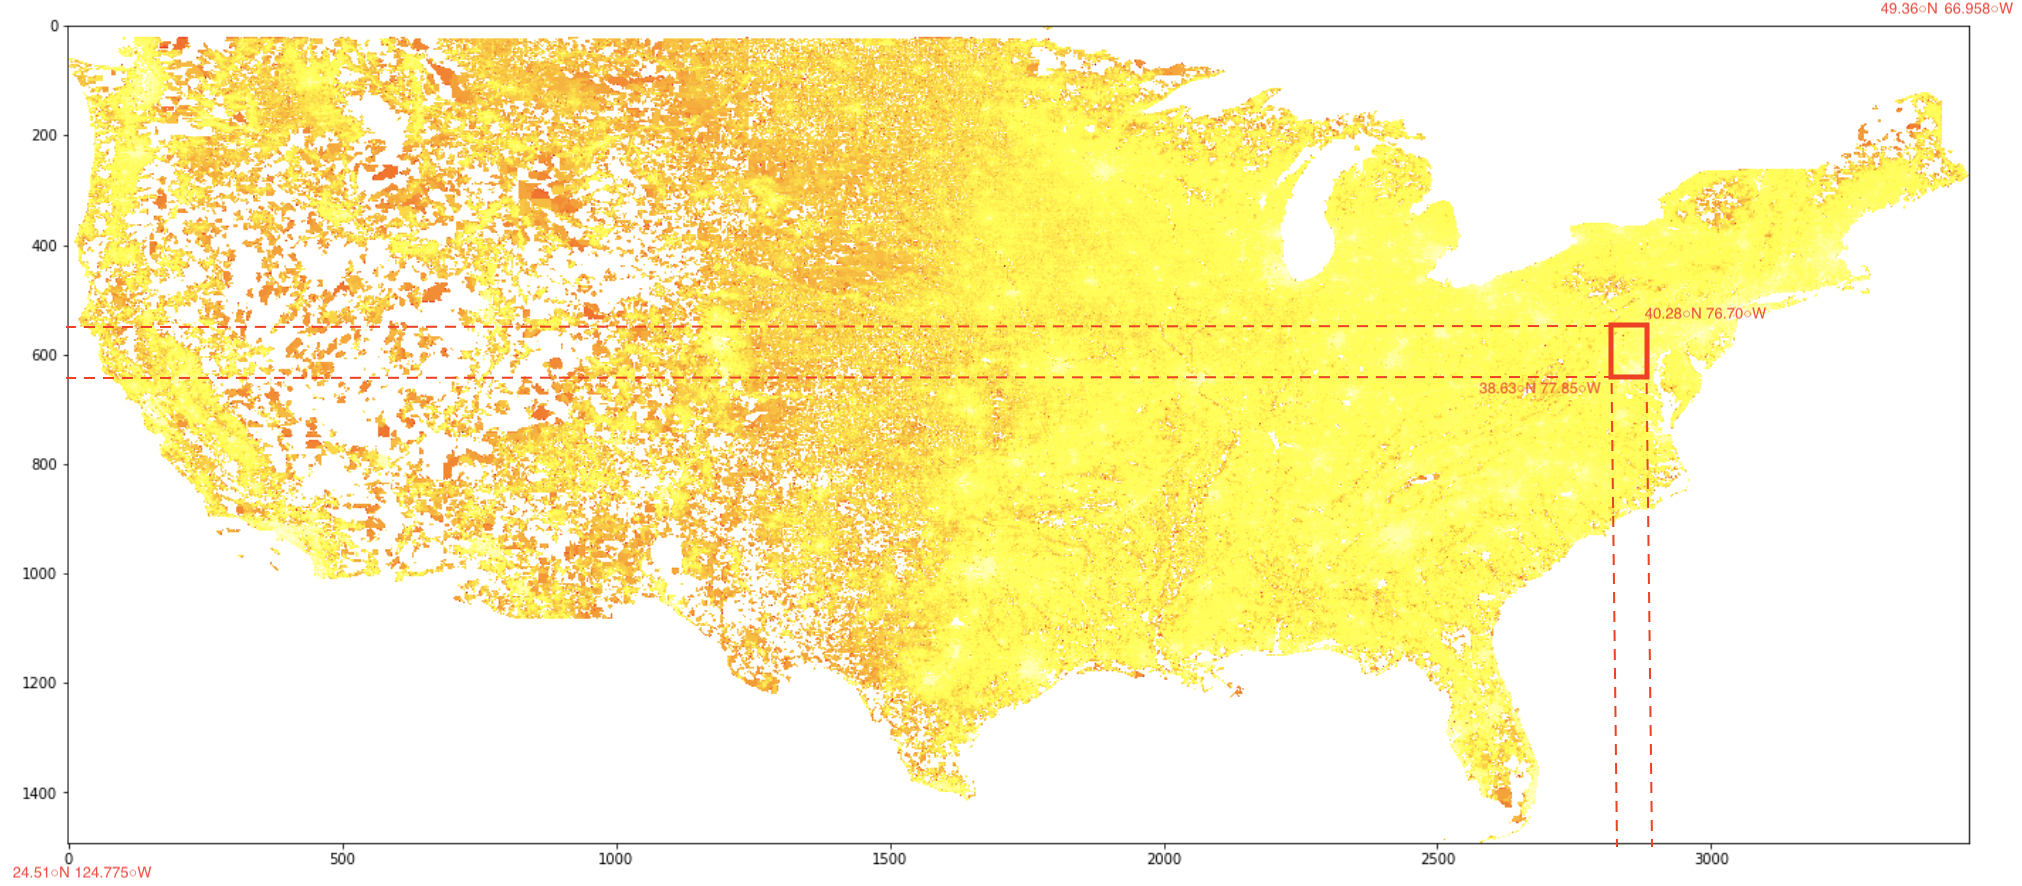
\includegraphics[scale=0.33]{heat_map.png}
\label{fig:training-area}
\caption{The sampling area}
\end{figure}

To overcome Google Engine’s downloading limitations we decided to obtain the imagery through a more flexible API that was available as open source code in a Github repository on the web\footnote{https://github.com/google/earthengine-api}. This not only gave us flexibility in terms of data usage, but also allowed us to select the dimensions, zoom level and resolution of our imagery,  to obtain an optimal data set according to our needs. Through various iterations in the data mining process we came to the conclusion that the extra time invested in obtaining would pay off during the modeling and evaluation phases. 

A total of 7000 images were downloaded, each image capturing a region of approximately 4 square kilometers. This selection was carefully chosen based on a compromise between our need to cover the selected training/testing region and an appropriate amount of image resolution that would allow the algorithms to identify details correctly. Each image is exactly 200 x 200 pixels with RGB color model.

We let the grids of satellite images be represented as the matrix $\theta$, where for every $P^{i,j}$  in the population matrix there is an associated satellite image $\theta^{i,j}$. Conveniently our census region which contains the ‘ground truth’ values of population has a resolution of 1 square kilometer so each image can be easily mapped to our data frame. The total population count for each variable is calculated by multiplying the area in square kilometers in each area of intersection by the density of that variable in the underlying census block. Given that the population density matrix data has a fixed resolution we performed a series of tests to determine the accuracy of our ground truth matrix. For practicality we performed this test for the two states that specifies their extent strictly in terms of lines of latitude and longitude, rather than rivers, mountain divides, or other geographical features: Colorado and Wyoming. The results of this test are plus minus 4\% of the expected population and therefore we conclude that the nature of our population matrix contributes to our sources of irreducible error.

With this in mind we estimate the population of our area of interest to be 6,859,980. Our data was randomly split in 80\% training and 20\% validation data ($70\%$-$30\%$ on one occasion). To increase variability, we did this splitting independently for each model we built.

\newpage
Mostly throughout this project, we viewed our problem as a multi-type classification task, sorting the images into different population density intervals:

\begin{figure}[ht]
\center
\begin{tabular}{ |c|c| } 
\hline
Population interval & Number of images\\
\hline
0-1& 154\\ 
1-10& 782\\ 
10-50& 2813\\
50-100& 908\\
100- 500& 1294\\
500-1000& 529\\
1000-2000& 401\\
2000-11000& 119\\
Total& 7000\\
\hline
\end{tabular}\vspace{0.5cm}
\centering
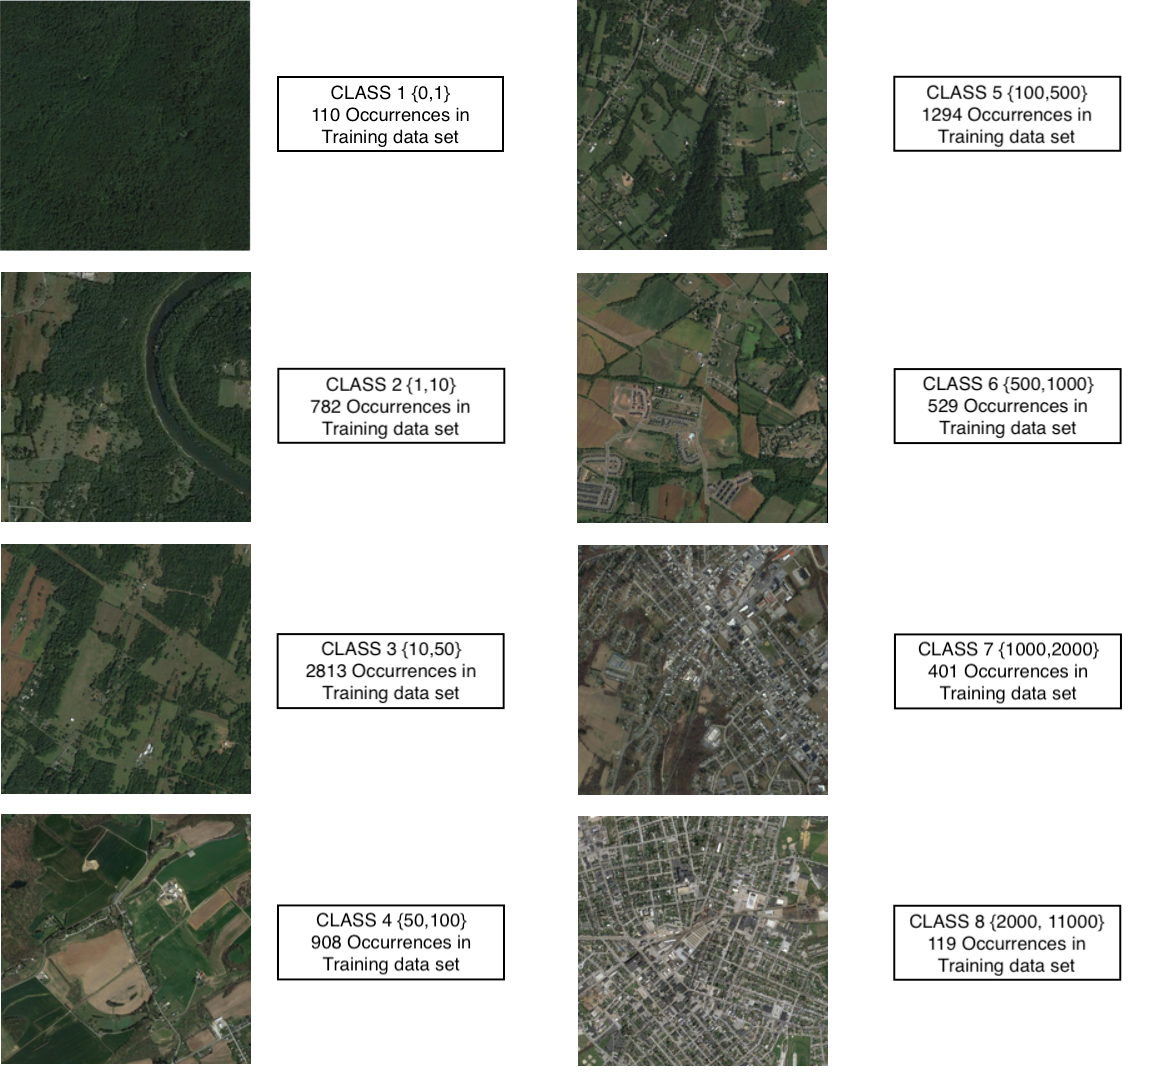
\includegraphics[scale=0.5]{samples.png}
\caption{Population intervals and the number of corresponding images in our dataset.}
\end{figure}\newpage


\section{Modeling and evaluation}
Our goal in this section is to describe the models we built and to demonstrate that they are capable of extracting predictive value from our data, that is, our models provide a non-unit lift compared to random guessing.

\subsection{Logistic regression}
Our first approach to establish a baseline was to use a One vs Rest classifier using Logistic Regression for each of the classes using the method described in the corresponding class Lab. This approach required the 7000 200x200 RGB images to be vectorized and the result for each is a vector with 120 000 entries, each entry taking values between 0 and 255.

After processing each image and looking up their labels in the census data, the result was a 120 001 by 7000 DataFrame. Being massive, this DataFrame required us to use a 64 CPU cluster in order to complete our task. Also, in order to make the training faster, we did a 70-30 split between training and testing sets, thereby reducing the training set compared to our other models running on GPU-s.

Once the training was complete, we plotted the validation set confusion matrix for our classifier:

\begin{figure}[ht]
\centering
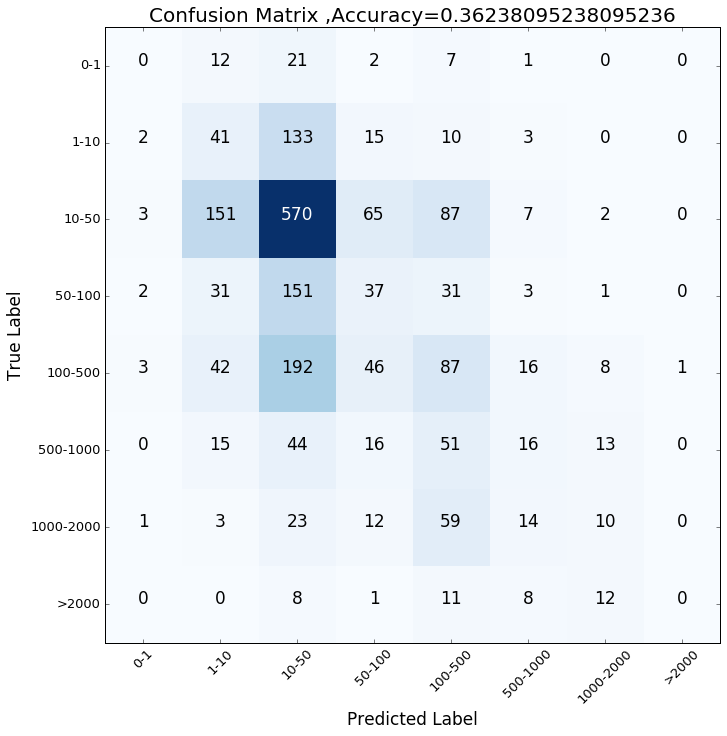
\includegraphics[scale=0.35]{yassine_cm.png}
\end{figure}

We did not have high expectations for this approach, however if we consider random guessing as our baseline, this model seems to perform somewhat better on average (36.2\% validation accuracy). 

\subsection{Convolutional Neural Network from scratch}
This section describes the development of a Deep Convolutional Neural Network from scratch, and fully coded in Python using the State-of-the-art Deep Learning framework, Tensorflow.

In this case, this networks has been coded to perform a \textbf{regression} problem, not a classification. For measuring the accuracy, however, the same population intervals have been used in order to define if a given prediction lies in its correct interval or not.

 \subsubsection{Architecture}
 
 The high-level architecture of the network is described below:
 \begin{enumerate}
\item \textbf{Convolutional layer 1:} three channels as input, 8 feature maps as output. ReLU activation function. Kernel size of 3x3. Stride of 1x1.
\item \textbf{Maxpooling layer:} Pool size and stride of 2x2.
\item \textbf{Convolutional layer 2:} 16 feature maps as output. ReLU activation function. Kernel size of 3x3. Stride of 1x1.
\item \textbf{Maxpooling layer:} Pool size and stride of 2x2.
\item \textbf{Convolutional layer 3:} 16 feature maps as output. ReLU activation function. Kernel size of 3x3. Stride of 1x1.
\item \textbf{Maxpooling layer:} Pool size and stride of 2x2.
\item \textbf{Convolutional layer 4:} 32 feature maps as output. ReLU activation function. Kernel size of 3x3. Stride of 1x1.
\item \textbf{Maxpooling layer:} Pool size and stride of 2x2.
\item \textbf{Reshape:} Flatten output from fourth convolutional layer.
\item \textbf{Fully connected layer 1:} 512 neurons. ReLU activation function.
\item \textbf{Fully connected layer 2:} 128 neurons. ReLU activation function.
\item \textbf{Output:} population estimation. One output.
 \end{enumerate}

The images fed into the network have been 200x200x3 (RGB) pixels, and in batches of 64 images randomly selected from the training set, and without replacement.
 
\subsubsection{Optimizers}
In order to perform the best possible prediction, different optimizers have been tested. These are:
\begin{itemize}
\item \textbf{Adadelta optimizer:}\footnote{http://ruder.io/optimizing-gradient-descent/index.html\#adadelta} It is an extension of Adagrad that seeks to reduce its aggressive, monotonically decreasing learning rate. Instead of accumulating all past squared gradients, Adadelta restricts the window of accumulated past gradients to some fixed size [1].
\item \textbf{Adam optimizer:}\footnote{http://ruder.io/optimizing-gradient-descent/index.html\#adam}
 Stands for Adaptive Moment Estimation, and it is a method that computes adaptive learning rates for each parameter. In addition to storing an exponentially decaying average of past squared gradients like Adadelta and RMSprop, Adam also keeps an exponentially decaying average of past gradients, similar to momentum [2].
\end{itemize}


Different learning rates have been tested on both optimizers, and the final rates used have been: $\eta = 0.1$ for Adadelta, and $\eta = 0.001$ for Adam.

\subsubsection{Training details}
Different training techniques have been applied in order to compare the performances and choose the best. These are:
\begin{itemize}
\item \textbf{Oversampling:} Since the amount of images in every class defined for accuracy is not equal, an oversampling technique has been perform in order to uniformly select images from all classes when creating the random training batch at every training iteration.
\item \textbf{Similar distribution in train and test sets:} In order to have a less biased training set, the split between training and test images has been perform in such a way that both interval distributions are similar.
\end{itemize}
 
With respect to the software and hardware equipment, Tensorflow 1.3 and CUDA 8 have been running using NVIDIA GTX 1080 GPU.
 \newpage 
 \subsubsection{Results}\vspace{-0.5cm}
 
 \begin{figure}[ht] 
  \begin{minipage}[b]{0.5\linewidth}
    \centering
    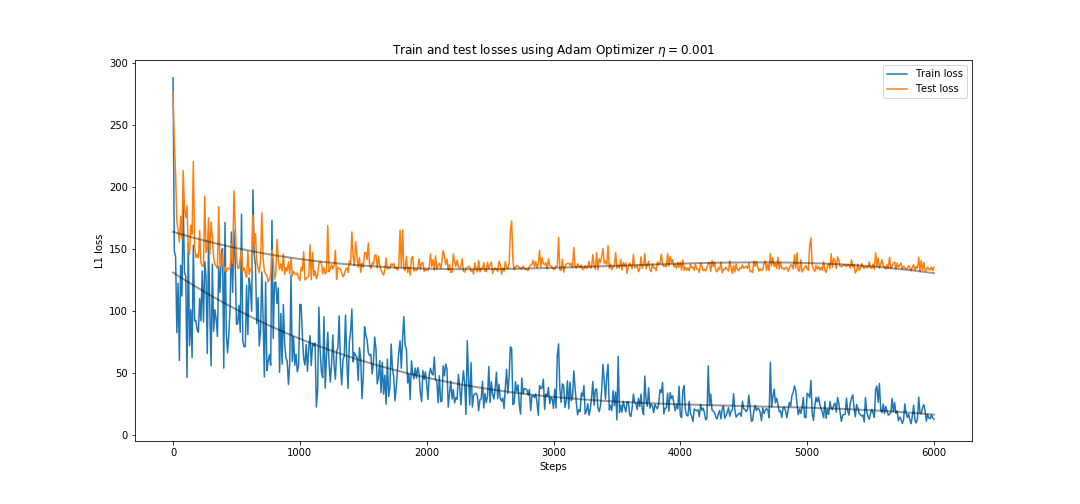
\includegraphics[width=1.1\linewidth]{loss_adam.png} 
    \caption{Loss with Adam} 
  \end{minipage}
  \begin{minipage}[b]{0.5\linewidth}
    \centering
    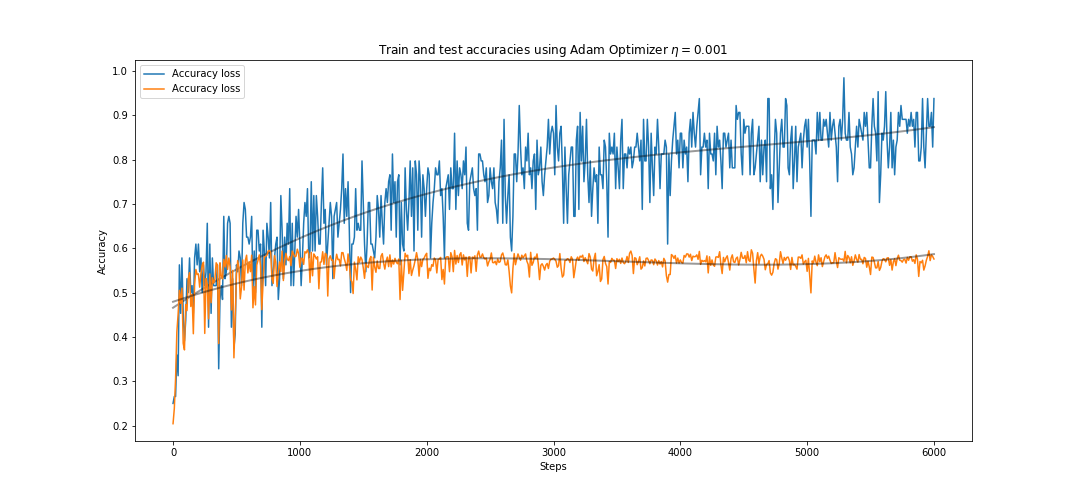
\includegraphics[width=1.1\linewidth]{acc_adam.png} 
    \caption{Accuracy with Adam}
  \end{minipage} 
  \begin{minipage}[b]{0.5\linewidth}
    \centering
    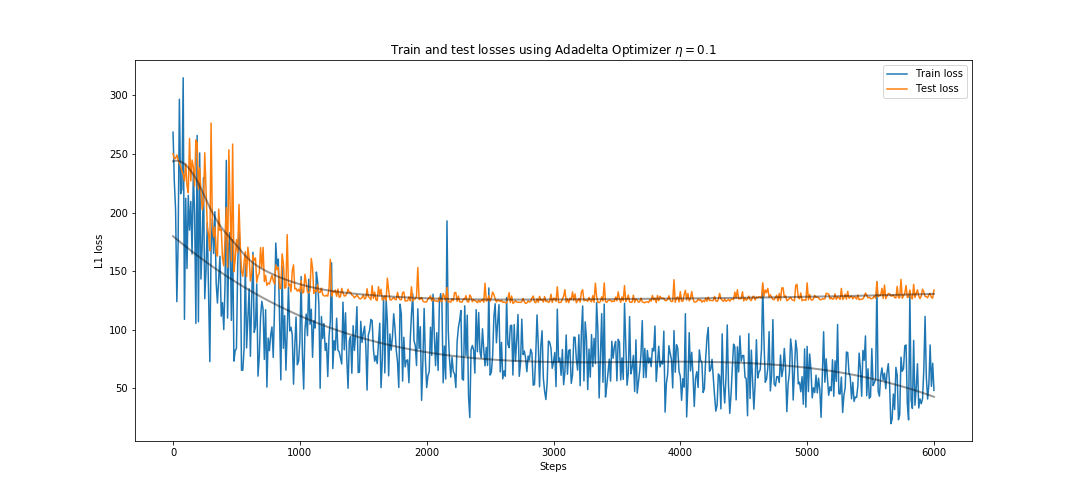
\includegraphics[width=1.1\linewidth]{loss_adadel.png} 
    \caption{Loss with Adadelta} 
  \end{minipage}
  \begin{minipage}[b]{0.5\linewidth}
    \centering
    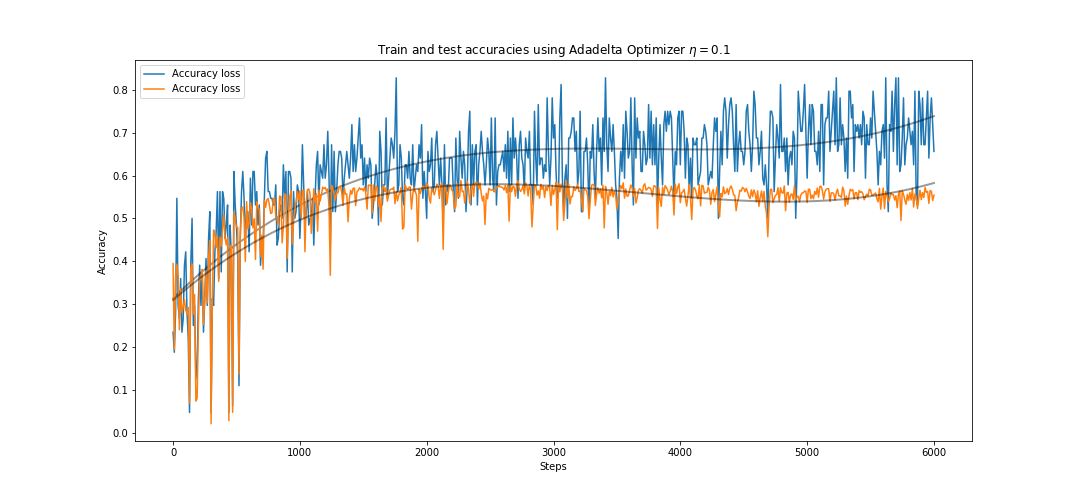
\includegraphics[width=1.1\linewidth]{acc_adadel.png} 
    \caption{Accuracy with Adadelta}
  \end{minipage} 
 \begin{minipage}[b]{0.5\linewidth}
    \centering
    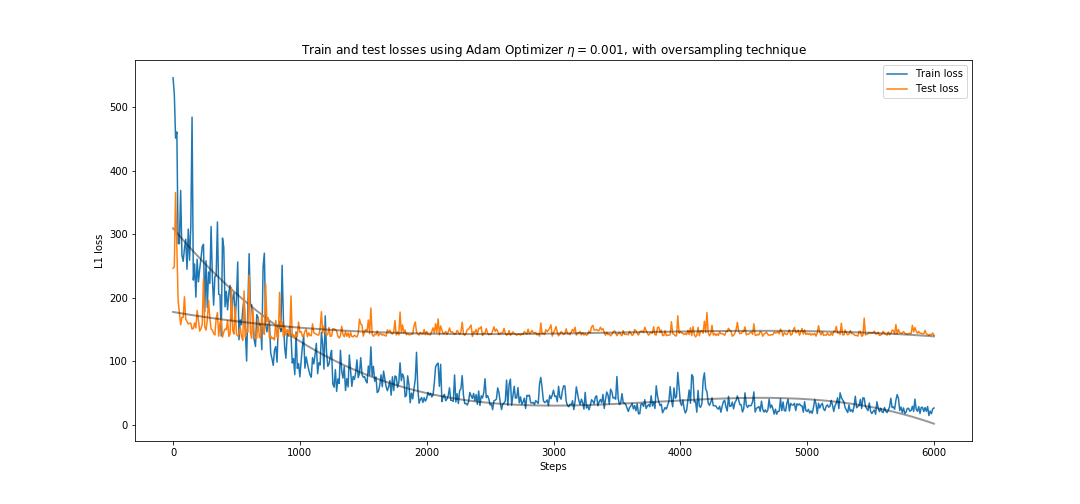
\includegraphics[width=1.1\linewidth, height = 3.8cm]{loss_adam_oversample.png} 
    \caption{Loss Adam oversampling} 
  \end{minipage}
  \begin{minipage}[b]{0.5\linewidth}
    \centering
    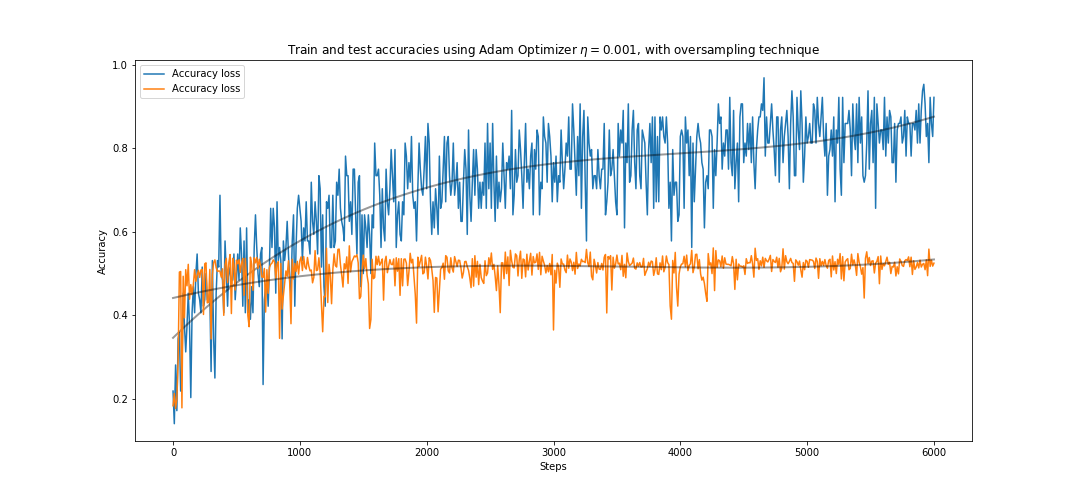
\includegraphics[width=1.1\linewidth, height = 3.8cm]{acc_adam_oversample.png} 
    \caption{Acc. Adam oversampling}
  \end{minipage} 
  \end{figure}

\begin{figure}
 
  \begin{minipage}[b]{0.5\linewidth}
    \centering
    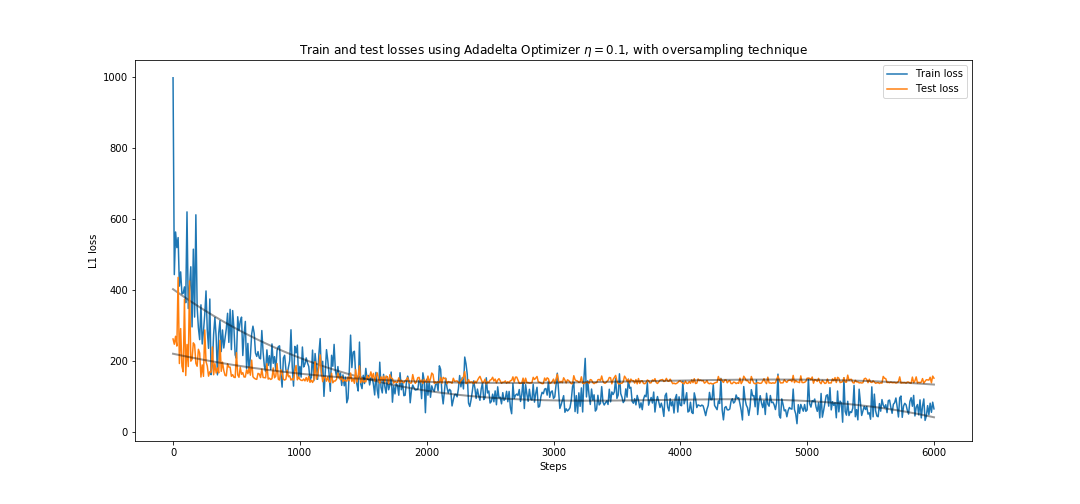
\includegraphics[width=1.1\linewidth, height = 3.8cm]{loss_adadel_oversample.png} 
    \caption{Loss Adadelta oversampling} 
  \end{minipage}
  \begin{minipage}[b]{0.5\linewidth}
    \centering
    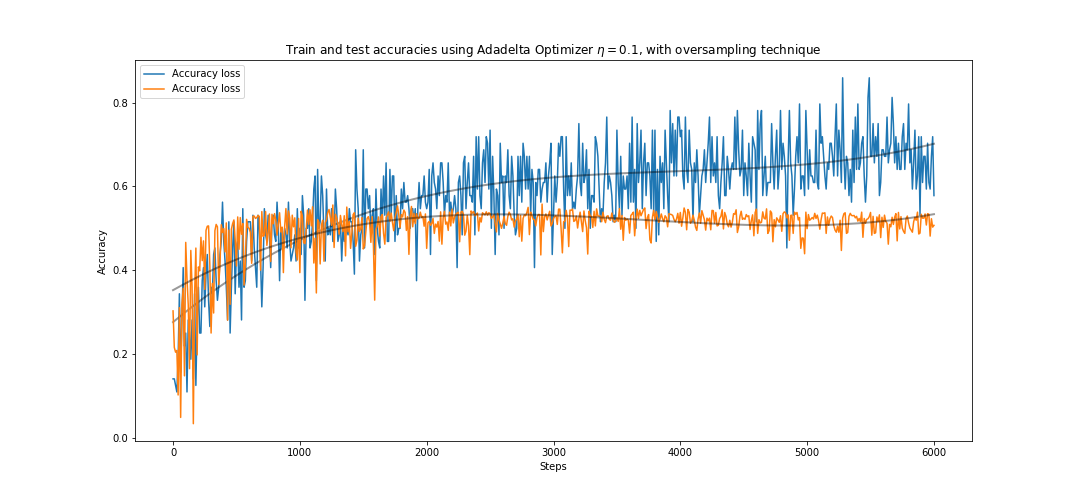
\includegraphics[width=1.1\linewidth, height = 3.8cm]{acc_adadel_oversample.png} 
    \caption{Acc. Adadelta oversampling}
  \end{minipage} 
\end{figure}

\newpage
\subsubsection{Conclusions}
As we can see from the results above, the best accuracies are achieved using both Adam and Adadelta optimizers (surprisingly) without oversampling, but splitting test and test sets keeping the similar interval distributions. 








\subsection{Pretrained VGG architecture}
The Vgg16 architecture is a 16 layer CNN developed for large scale image recognition by the Visual Geometry Group at the University of Oxford (\cite{SZ14}). This architecture won the ILSVRC-2014 ImageNet competition in 2014. We use the Keras version that has been obtained by directly converting the Caffe model provided by the authors\footnote{https://gist.github.com/baraldilorenzo/07d7802847aaad0a35d3, however, we use the modified version adapted to the Fast.ai course.}.


Vgg16 is designed to assign probability scores of an image belonging to 1000 different ImageNet categories. We finetune the network according to our population intervals, that is we use the ImageNet scores as features to predict our population intervals (so essentially we assign scores that a satellite image is a dog, cat, corn, ketchup, etc. and then use these scores as inputs for classification). After performing a random $80\%-20\%$ split between the training and validation set, we performed 30 training epochs using the ADAM\footnote{https://machinelearningmastery.com/adam-optimization-algorithm-for-deep-learning/} algorithm with learning rate $0.001$ and categorical cross-entropy as our loss function. This gave us validation accuracy of $62.29\%$ and validation loss $1.0054$. Moreover the confusion matrix on the validation set is plotted on the left of Figure \ref{fig:conf-mx-es}.
\begin{figure}[ht]
\centering
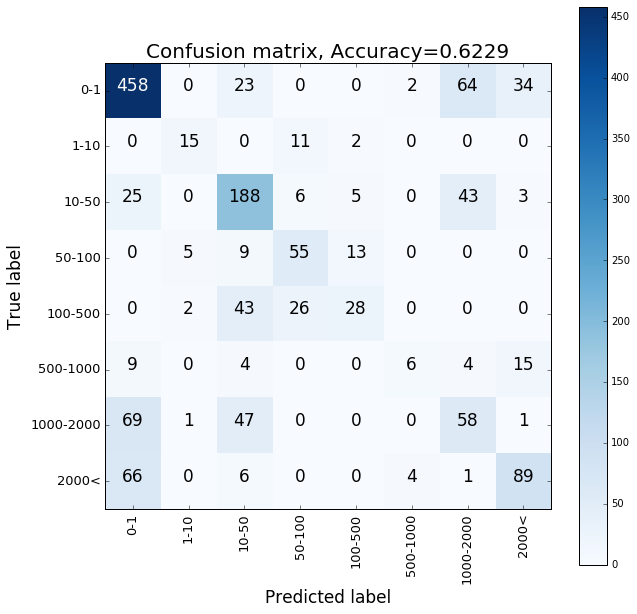
\includegraphics[scale=0.35]{conf_mx_Zsolt1.png} 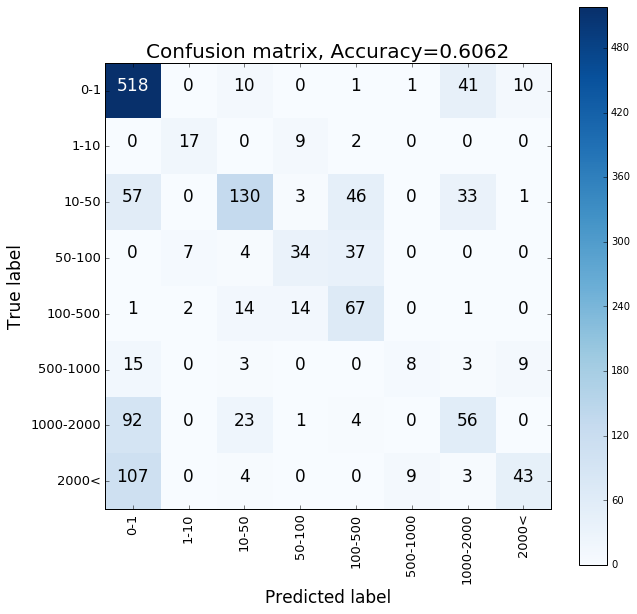
\includegraphics[scale=0.35]{conf_mx_Zsolt2.png}
\caption{Validation set confusion matrices for the finetuned Vgg16 (left) and with the last hidden layer retrained (right).}
\label{fig:conf-mx-es}
\end{figure}

To see if we can improve performance, we also attempted to retrain the last hidden layer of the model (using the finetuned model above, to avoid starting with random weights in the final layer, which would cause the retrained layer to quickly move a long way from its optimized ImageNet weights). This gave us a lower validation accuracy of $60.62\%$ and the validation set confusion matrix on the right of Figure \ref{fig:conf-mx-es}.

On several preliminary rounds, we have observed the validation accuracy fluctuating between $60-62\%$, which leads us to the conclusion that further training epochs would not improve our model.



\subsection{Comparison of our models}
To compare the accuracy of our models on an independent test set, we considered a balanced set of 168 images close to the area where our original sample was obtained. Since the set is balanced over the population intervals, the accuracy of random guessing is $12.5\%$. To test our models on a different terrain, we obtain a small balanced test set of 160 images from the San Francisco bay area. The accuracy results are summarized in Figure \ref{fig:accur-comp}.

\begin{figure}[ht]
\center
\begin{tabular}{ |c|c|c| } 
\hline
Model & EC & WC\\
\hline
RandomGuess & $12.5\%$ & $12.5\%$\\
LogReg& $23.81$ & $12.58\%$\\ 
CNNfromScratch & $43.26\%$ & $43.13\%$\\ 
Vgg16FineTune& $42.26\%$ & $32.5\%$\\
Vgg16Retrain& $45.83\%$ & $30.62\%$\\
\hline
\end{tabular}
\caption{Accuracies of our different models on the same test sets from the east coast (EC) and the west coast (WC).}
\label{fig:accur-comp}
\end{figure}

As expected, most models perform significantly worse on the geographical area different from that in the training set. Suprisingly, our hand built CNN performs comparably to the pretrained network (and even outperforms it on the west coast test set), which is something that would have been worth looking into further given more time. These accuracy figures (with one exception) nevertheless represent significant improvement over what one would expect from random guessing. We consider this as a successful proof of concept that it is indeed possible to extract information on the population of a particular region from satellite images taken from that area. It is worth remarking that the west coast test set involved certain areas of San Francisco itself where highly populated areas exist right next to a significant body of water. We speculate that this is extremely capable of confusing our model contributing to the lower accuracy figures as well for the LR and Vgg16 models.

\section{Deployment}
While we did not obtain high enough accuracy for reliable use, in this section we describe issues related to deployment after sufficient improvement has been achieved. After a successful validation of our models, deployment should be in the form of an automated software implementation, where decision makers can obtain the figure on the population of a particular area by simply feeding the neural network the corresponding satellite images.

However, every governmental agency using our model for decision making should be aware of the imperfection of our predictions. Accordingly, whenever human life depends on the results (e.g. evacuation planning, or disaster relief funds), the policymakers should make sure to have appropriate cushion built into their actions. To provide further security, the cautious user should use our models in conjunction with other techniques and be alerted by huge discrepancies. This of course applies to all other applications with, perhaps, less severe consequences.

As features of areas populated by humans, in particular overall architecture, change rather slowly over time, one would expect a well trained model to be robust over a long period of time. Of course, the model should go through revalidation or, perhaps, retraining from time to time. A natural point for this to occur are the census years, when labeled data becomes available.

Unless it is the explicit goal of using the model (e.g. in clandestine applications), one has to be aware that obtaining satellite images of people's properties raises obvious privacy issues. The respectful user should use a low enough resolution such that the details of individual's properties cannot be extracted from the image.

\section{Possible further directions}

There are many interesting questions arising in connection with using our models that we did not have the chance to investigate due to the lack of time and data acquisition difficulties.

For example, we could have looked at different (preferrably larger) training sets containing different terrains, e.g., training in California and testing on the east coast. We could have also tried to perform population estimates on foreign countries to see how well our models generalize. For example, it would have been interesting to predict the population of North Korea and see how the measurement would correlate with the official figure. We could have also used different population intervals to see if it increases accuracy. Finally, the models used and implemented are quite standard and general purpose. It could be interesting and worth exploring to implement Neural Networks architectures more adapted to our problem.

\appendix
\section{Contribution of each team member to the project}
\subsection{Yassine Kadiri}
First found the article when looking for a project idea. Found the datasources (US Census and satellite imagery). Processed the US census data (ASCII File) in order to display it as a DataFrame and keep record of all the other parameters included in the file. Vectorized the images and labeled them. Implemented the One-vs-all classifier. Wrote the first version of the project proposal and the Logistic Regression section in this report. Contributed to the Possible further directions section.
\subsection{Santiago Novoa}
My contribution on this project was twofold.
First I worked on the data mining, creating the dataset by taking a semi processed census matrix, and interpreting the data to produce meaningful results we could use. With this as a basis I worked on creating a method for obtaining the satellite imagery that completes the data set, and matches the census matrix.
Also, I contributed secondarily on the implementation of the CNN in Tensorflow for this project. Lastly, I wrote the data section of the report.
\subsection{Zsolt Pajor-Gyulai}
Researched the paper \cite{RHD17}, when the project proposal came up. Worked on the write-up of the project proposal. Learned how to use the Vgg architecture (and how to do any sort of deep learning in the first place) from the online Fast.ai course. Built the Vgg model and wrote the corresponding section in this write-up. Wrote the first version of the 'Summary', 'Business understanding', and 'Deployment' sections of this write-up.

\subsection{Manuel Serrano}
Worked on the data mining and feature engineering: imagery scraping from Google Maps using Python API, census data cleaning and preparation to accurately match population data with corresponding satellite image. Also developed CNN in pure Tensorflow from scratch. Learnt different State-of-the-art types of optimizers and training techniques in Deep Learning and implemented in raw Tensorflow to get real results.

\begin{thebibliography}{9}

\bibitem[BDYPHN06]{BDYPHN06} \textsc{D. Balk, U. Deichmann, G. Yetman, F. Pozzi, S. Hay, A. Nelson} \textit{ Determining global population distribution: methods, applications, and data.} Advances in parasitology, Vol 62, p119-156 (2006)

\bibitem[L96]{L96} \textsc{J. Long}\textit{ Postcensal population estimates: States counties and places.} Indirect Estimators in US Federal Programs, p59-82, Springer (1996)

\bibitem[PF13]{PF13} \textsc{F. Provost, T. Fawcett} \textit {  Data science for business: [what you need to know about data mining and data-analytic thinking]}. Sebastopol, Calif.: O'Reilly.


\bibitem[RHD17]{RHD17}  \textsc{C. Robinson, F. Hohman, B. Dilkina}\textit{ A Deep Learning Approach for Population Estimation from Satellite Imagery.} arXiv preprint arXiv:1708.09086 (2017)

\bibitem[SZ14]{SZ14} \textsc{K. Simonyan, A. Zisserman} \textit{ Very Deep Convolutional Networks for Large-Scale Image Recognition} arXiv preprint arXiv:1409.1556
\end{thebibliography}
\end{document}